%======================================================================================== 
%Preamble. Latex needs all this stuff to work, but it doesn't appear in your document.
\documentclass{article}[12pt]
\usepackage{geometry}                
\usepackage{graphicx}
\usepackage{amsmath}
\usepackage{amssymb}
\usepackage{float}
\floatstyle{plain}
\usepackage[]{microtype}
\usepackage{listings}
\lstset{
    literate={~} {$\sim$}{1}
}
\usepackage{color}
\usepackage{epstopdf}

\usepackage{lipsum}
\newcommand{\eqname}[1]{\tag*{\bf #1}}% Tag equation with name
%\DeclareGraphicsRule{.tif}{png}{.png}{`convert #1 `dirname #1`/`basename #1 .tif`.png}
\usepackage{hyperref}
\hypersetup{
    colorlinks=true,
    linkcolor=blue,
    filecolor=magenta,      
    urlcolor=blue,
    citecolor={blue}
    }
    
\usepackage[backend=biber, style=authoryear, uniquename=false,doi=false,isbn=false, url=false, giveninits]{biblatex}
\usepackage[utf8]{inputenc}
\usepackage[toc, section=section]{glossaries}
\addbibresource{FYP_references.bib}

\makeglossaries
\newglossaryentry{CNCC}
    {name = CNCC,
    description = {Cranial Neural Crest Cell}
}
\newglossaryentry{EPO}
    {name = EPO,
    description = {Enredo, Pecan, Ortheus pipeline algorithm used by Ensembl to construct a multiple sequence alignment from sequences generated from pairwise whole-genome alignments}
}
\newglossaryentry{FOXC1}
    {name = FOXC1,
    description = {Forkhead Box C1 Gene}
}
\newglossaryentry{GRN}
    {name = GRN,
    description = {Genetic Regulatory Network}
}
\newglossaryentry{GTR}
    {name = GTR,
    description = {General Time-Reversible model of nucleotide substitution}
}
\newglossaryentry{HAR}
    {name = HAR,
    description = {Human-Accelerated Region}
}
\newglossaryentry{LRT}
    {name = LRT,
    description = {Likelihood Ratio Test}
}
\newglossaryentry{MSA}
    {name = MSA,
    description = {Multiple Sequence Alignment}
}
\newglossaryentry{NCC}
    {name = NCC,
    description = {Neural Crest Cell}
}
\newglossaryentry{SSREV}
    {name = SSREV,
    description = {Strand-symmetric time-reversible model of nucleotide substitution}
}

%\usepackage{biblatex}
%==========================================================
% My title, name, and date
\title{\emph{Cis}-regulatory enhancer of \emph{FOXC1} gene associated with jaw development shows accelerated evolution in \emph{Homo sapiens}}
\author{Esta V. Shrewsbury}
%==========================================================

\setlength{\parskip}{1em}

\begin{document}

\maketitle

\addcontentsline{toc}{section}{Abstract}
\section*{Abstract}

The Cranial Neural Crest Cell (CNCC) pathway is involved in craniofacial development in amniotes. This pathway is highly conserved and plays a key role in determining many anatomical \& physiological phenotypes during amniote development. Geometric morphometric studies of primate skulls show that human jaws have undergone accelerated evolution following our divergence from chimpanzees. This suggests there are genes or sequences linked to the CNCC pathway that also show accelerated evolution in the human genome. The aim of this project was to test for acceleration in the \emph{cis}-regulatory enhancer of the \emph{FOXC1} gene. This sequence was selected from a comparative gene expression study which found evidence of human-biased \emph{FOXC1} expression in human neural crest cell cultures (compared to chimpanzees). A meta-analysis was carried out on an Multiple Sequence Alignment (MSA) for this regulatory sequence and 23 predicted primate homologs. The results of this analysis showed no significant evidence for evolutionary conservation in this aligned sequence for non-human primates, but a few coordinates of the human sequence showed accelerated evolution. Further analysis may help to build a better understanding of the genetic basis behind the accelerated rate of evolution in human jaw development.
\newpage

\tableofcontents

\newpage

\printglossary

\newpage

\addcontentsline{toc}{section}{Introduction}
\section*{Introduction}

Humans show many uniquely derived anatomical and behavioural features that make us stand out from other primates. Unlike other apes, humans have flatter faces with a characteristic round skull shape, less-pronounced brow ridges and significantly reduced prognathism \parencite{Martinez2009}. Geometric morphometric analyses on primate skulls have highlighted these features as the key components of our craniofacial anatomy that show the greatest variation between humans and other primates \parencite{Raia2018}. This study has also shown that human jaws have undergone an accelerated rate of evolution following our divergence from chimpanzees.

The genetic basis for interspecific craniofacial differences is still poorly understood as the genetic pathways responsible are complex and highly conserved. Since humans share over 95\% of our DNA with chimpanzees \parencite{Suntsova2020, Varki2005}, this limits our search down to the remaining divergent ~5\% of the genome that must explain all of the phenotypical differences between humans and chimpanzees. The majority of these varied sequences are non-coding regulatory genes \parencite{Franchini2017}.

The Neural Crest Cell (\Gls{NCC}) pathway is a Genetic Regulatory Network (\Gls{GRN}) that controls the induction and migration of the NCC population at key points during vertebrate embryogenesis \parencite{Huang2004, Li2009}. \Glspl{NCC} are a temporary group of multipotent stem cells that can differentiate into many diverse cell lineages, the Neural Crest is established following induction via the \emph{BMP}, \emph{Wnt} and \emph{FGF} cell signalling pathways. This activates expression of various transcription factors, such as \emph{Snail}/\emph{Slug}, \emph{Foxd3} \& \emph{SoxE}, which subsequently the borders of the NCC populations that act as precursors to various tissues – e.g., the mesenchyme differentiates into osteoblasts (bone), myocytes (muscle), and chondroblasts (cartilage) etc. \parencite{Huang2004, Kulesa2010}

Depending on their position along the anterior-posterior axis of the developing organism during \Gls{NCC} induction, the cell lineages will follow one of four different functional pathways \parencite{Huang2004}. These are the cranial, trunk, vagal \& sacral, or the cardiac neural crest. The \Glspl{CNCC} will migrate in a species-specific pattern along the dorso-lateral axis of the head thus determining the craniofacial mesenchyme \parencite{Kulesa2010, Bronner2012, deLeon2007}.

Genetic studies focused on human evolution have coined the term Human Accelerated Regions (HARs) applying to sequences within the human genome that are conserved in vertebrates but show significant nucleotide divergence in humans \parencite{Gittelman2015, Bird2007, Hubisz2014}. These regions were identified through comparative analyses between human and chimpanzee genomes. This study tests for these \Gls{HAR} requirements in a multiple sequence alignment of the \emph{cis}-regulatory sequence the \emph{\Gls{FOXC1}} gene, although I focused specifically on primates.

This gene was identified in a comparative study between cultured human \& chimpanzee \Glspl{CNCC} and their respective gene expression profiles \parencite{Prescott2015}. This study showed that \emph{FOXC1}, along with multiple other genes linked to the CNCC pathway, showed significantly higher expression in human CNCCs than in chimpanzee CNCC – described as human-biased activity. The increased expression of \emph{FOXC1} in human CNCC was subsequently linked to a \emph{cis}-regulatory enhancer sequence located downstream from \emph{FOXC1} in the human chromosome 6.

\emph{Cis}-regulatory elements are non-coding regions of the genome that regulate the expression of neighbouring by acting as binding sites for transcription factors, this promotes the transcription of the associated gene \parencite{deLeon2007, Prescott2015, Wray2007}. 

The initial hypothesis was \Gls{CNCC} pathway associated genes that showed species-biased activity in humans or chimpanzees will have \emph{cis}-regulatory enhancers that may show evidence for accelerated evolution when compared to homologous sequences in primates. This could partially explain the genetic basis for accelerated evolution in human jaw development. 

\addcontentsline{toc}{section}{Methods}
\section*{Methods}

Genomic transcripts for the chosen sequence (chr6: 1744897 – 1745096) were obtained using the Ensembl genomic database \parencite{Ensembl}. An \Gls{MSA} was constructed with Ensembl, containing the initial 200bp human sequence and 23 non-human primate homologs (as predicted by the \Gls{EPO} alignment algorithm automated by the Ensembl database). Ensembl release 104 introduces gaps using the EPO pipeline therefore the MSA was 236bp long although each individual primate sequence ranged around 200bp (see \hyperref[sec:supp]{Supplementary Material}). The EPO-alignment and the representative phylogenetic tree were downloaded in FASTA \& Newick formats, respectively.

Twelve of the total 24 primates selected for the alignment were noted as having low-quality alignment assembly. Listed: Sooty Mangabey, Drill, Pig-Tailed Macaque, Black Snub-Nosed Monkey, Golden Snub-Nosed Monkey, Ma’s Night Monkey, White Faced Capuchin, Bolivian Squirrel Monkey, Tarsier, Greater Bamboo Lemur, Coquerel’s Sifaka \& Bushbaby.

MSA analysis was carried out using the software R \parencite{R} and the packages Biostrings \parencite{Biostrings}, rphast \parencite{Rphast} \& ape \parencite{Ape}. The rphast package was the key component for this analysis as it allowed us to test for the likelihood of conservation or acceleration within an MSA using phyloP tests.

The phyloP tests require a neutral model of evolution as the null hypothesis. Therefore, we ran a phyloFit test for the MSA to set this model (object class: tm). The parameters set for this were nrates- 4, model- SSREV, EM- TRUE \parencite{Gittelman2015}. Here we used the phylogenetic tree provided with the Ensembl EPO-primate alignment in Newick format to set the neutral tree model (see Figure \ref{fig1}).

%Figure 1
\floatstyle{plain}
\restylefloat{figure}
\begin{figure}[H]
\centering
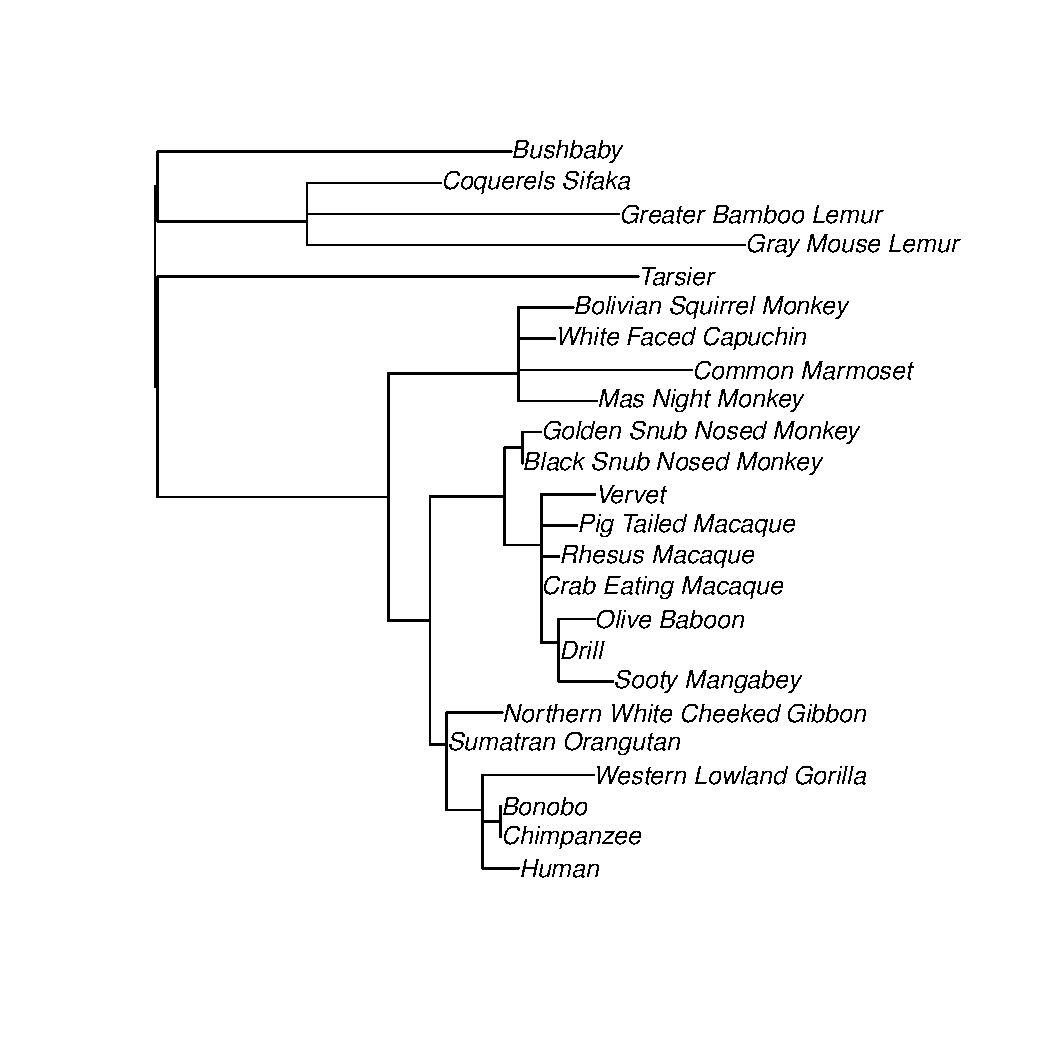
\includegraphics[width=12cm]{neutral_tree.pdf}
\caption{Phylogenetic tree of 24 primate \Gls{EPO}-alignment of the \emph{FOXC1} \emph{cis}-regulatory enhancer sequence. Constructed using the neutral model (phyloFit - estimating branch lengths) and the R package ape \parencite{Ape}}
\label{fig1}
\end{figure}

The \Gls{SSREV} model is a variant of the \Gls{GTR} model of nucleotide substitution. The SSREV model, in contrast, takes into account the limitations of double-stranded DNA thus the base frequency on one strand changing will directly affect the complementary base frequency on the opposite strand. This model only requires four substitution rate categories (nrates) whereas the normal GTR model requires six \parencite{PhyloP, Gittelman2015}. The neutral model set by phyloFit assumes no selection therefore all nucleotide variation should be sufficiently explained by neutral genetic drift.

Three consecutive phyloP tests were carried out, each outputs a matrix of p-values and scores according to the specified mode. These correspond to the coordinates in the MSA and determine the likelihood of the apparent nucleotide variation fitting the neutral model (previously set with phyloFit) – here the critical value is p-value $<$ 0.05. All three tests used the \Gls{LRT} scoring method - this adds a column for Lnl ratio, which is the ratio of likelihood scores between the two models (i.e., the neutral and the alternative model – mode options: NNEUT, CON, ACC). The Lnl ratio and associated p-values are combined into a score column as plotted in Figure \ref{fig2} (see \hyperref[sec:supp]{Supplementary Material} phyloP test results).

The first test included the full primate alignment and the previously constructed neutral model (phyloFit). Here we set the mode parameter to non-neutrality (NNEUT) to test for significant deviation at every coordinate in the alignment from the neutral model – this consequently suggests that the assumption of no selection has been violated, although this could be either evidence for conservation or acceleration in the NNEUT test.

The second phyloP test was run for a subset of the MSA excluding humans. This phyloP test uses the mode conservation (CON). The alternative hypothesis for this test assumes that the 23 primates in this alignment show significantly less nucleotide variation between species than is expected in the neutral alignment – this could suggest negative/purifying selection to decrease nucleotide variation.

The third and final phyloP test used the full alignment, the mode acceleration (ACC) and the parameter subtree- humans. Significant p-values for this test may indicate positive/directional selection due to the introduction of a selective pressure in our recent evolutionary history.

\addcontentsline{toc}{section}{Results}
\section*{Results}
 
Three genomic positions in the entire primate alignment showed significant p-values for the NNEUT phyloP test. This indicates the nucleotide variation observed at those positions (for all primates in this alignment) could not be sufficiently explained by the neutral model. Interestingly, the non-neutral coordinates were located within approximately 20bp of each other – my initial thoughts were that this region could be functionally important, i.e., as a binding site, but further testing is required to explore this hypothesis. (Figure \ref{fig2})

The phyloP test for conservation in the non-human primate subset did not show any significantly conserved coordinates in the sequence. This is one of the requirements for a defined \Gls{HAR} therefore this confirms that this 200bp \emph{cis}-regulatory sequence is not unique to humans and may have undergone rapid evolution in other branches of the primate family tree – as suggested by the NNEUT results.

The phyloP test for human-specific acceleration showed significant p-values at two coordinates located at either end of the sequence. These positions do not overlap with the non-neutral coordinates identified in the full primate phyloP test (NNEUT). 

%Figure 2
\floatstyle{plain}
\restylefloat{figure}
\begin{figure}[H]
\centering
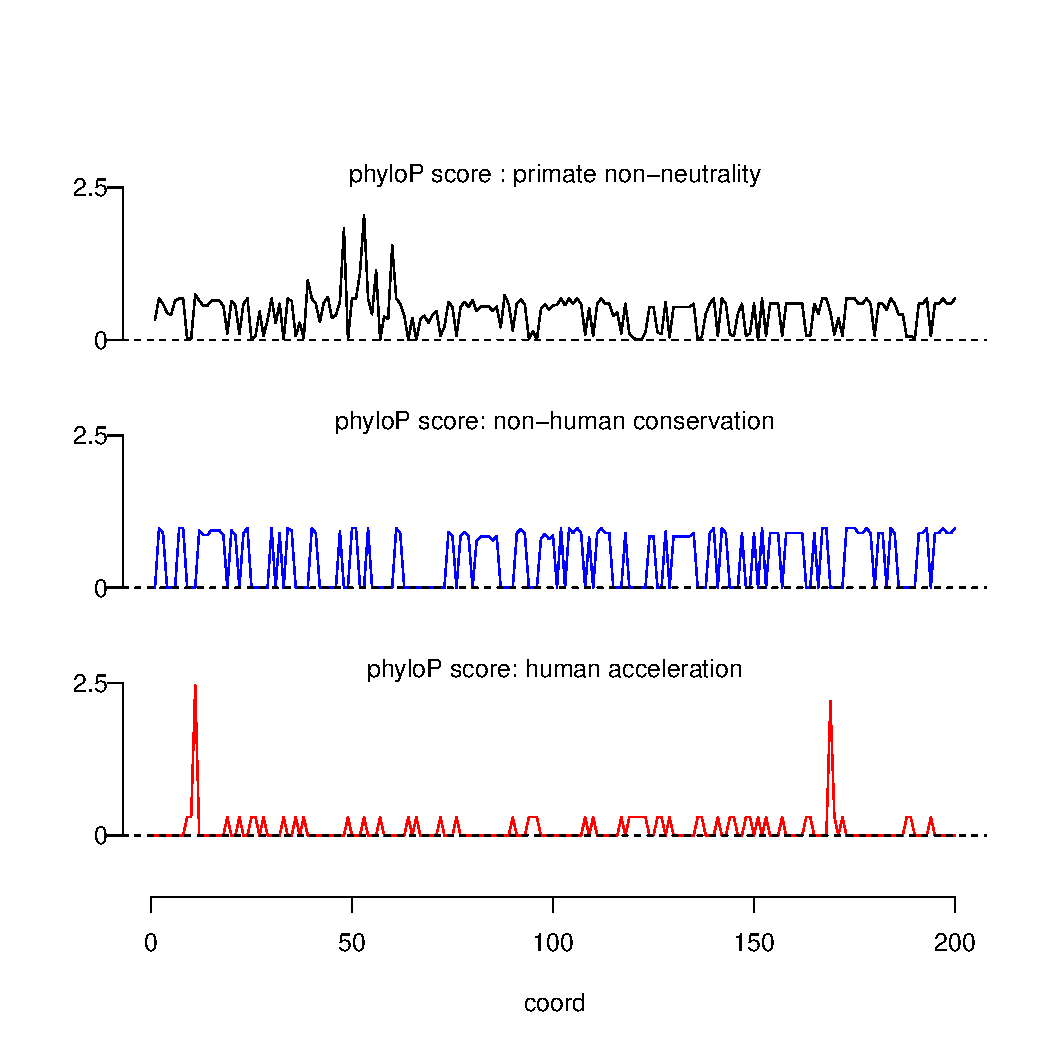
\includegraphics[width=12cm]{compare_phyloP.pdf}
\caption{Plot of phyloP scores for NNEUT, CON and ACC tests described in Methods. The x-axis "coords" corresponds to the base-pair within the primate MSA. This graph shows the significant peaks in the NNEUT and human ACC phyloP tests, the non-neutral coordinates are located within ~20bp of each other and do not overlap with the accelerated coordinates of the human sequence. The non-human primate CON phyloP results were not significant at any sequence coordinate. This graph was made using the plot.track function provided by the rphast package \parencite{Rphast}}
\label{fig2}
\end{figure}

The results of these tests suggest that this \emph{cis}-regulatory sequence is not unique to humans as a target of evolution as it does not fulfil the conservation requirements of a \Gls{HAR}. This implies that this sequence may be involved in interspecific craniofacial variation for other primate species, we could identify these branches by carrying out further phyloP testing for different subtrees of the primate alignment. Since human-accelerated coordinates of the sequence did not show any significant non-neutrality in first phyloP test, it is likely that those coordinates are not accelerated in any other primates and, by extension, the coordinates of non-neutrality are consistent for multiple species in the alignment.

Since I only analysed an \Gls{MSA} for a single reference sequence, the results for each phyloP test were calculated for each base-pair rather than for extended sequences so there is a definite risk of exaggerating the importance of the test results for specific coordinates. For example, I have made the assumption for this non-coding sequence that the impact of nucleotide variation on functionality (i.e., as a binding site) is the same across the entire sequence when it is possible that mutations at some coordinates are silent and thus may be misinterpreted as non-neutral or accelerated in phyloP tests. This highlights the limitations of a meta-analysis such as this, expression data is often unavailable for less well-known (and therefore less studied) genes which, unfortunately, includes many genes involved in \Gls{CNCC} pathway. Invasive gene expression studies on developing human embryos are obviously highly unethical so the process of mapping out complex \Glspl{GRN} (such as the CNCC pathway) in human and chimpanzee development to their corresponding phenotypes is incredibly difficult. 

Therefore, this meta-analysis attempts to bypass this gap in our understanding of \emph{FOXC1}’s involvement in human jaw development but, consequently, this means I cannot realistically prove that our chosen regulatory sequence explains the accelerated rate of evolution in human jaws.

As indicated by \cite{Prescott2015}, there are many regulatory sequences linked to \Gls{CNCC} genes that vary between humans and chimpanzees so a useful extension of this study would be to concatenate a selection of these sequences in a single \Gls{MSA} and carry out similar analyses. This concatenated MSA would string multiple different regions for the same species onto one large alignment, subsequent phyloP tests could be altered to output p-values corresponding to an entire sequence rather than for individual bases thus allowing one to candidate sequences for further analysis. This, however, has the disadvantage of losing the level of detail seen in our base-wise phyloP tests.

\addcontentsline{toc}{section}{Discussion}
\section*{Discussion}

The presence of a bony, hinge-like jaw is a characteristic feature of amniotes and is often classified as a key synapomorphy in phylogenetic studies \parencite{Franchini2017}. While the evolutionary origin of pharyngeal jaws (the ancestral pre-cursors to amniote jaws) is still highly debated, it is generally accepted that mammal, bird \& reptilian jaws are homologous \parencite{Kulesa2010}. This has allowed scientists to draw conclusions on human and primate jaw development using evidence based on developmental gene-expression studies on mice and chick embryos \parencite{Huang2004, Kulesa2010, Varki2005}. Therefore, the deeply embedded \Glspl{GRN} that control jaw development in primates are fundamentally the same. Most of the genes known to be involved in these pathways are highly conserved and thus differentiate very little between species \parencite{Bird2007} – despite this, primate jaws still show a significant level of morphological variation.

The main \Gls{GRN} responsible for jaw development, and thus interspecific jaw variation, is the \Gls{CNCC} pathway \parencite{McLean2011}. This pathway is a complex cascade of interacting transcription factors and other regulatory elements that establish a strictly-controlled spatial pattern of gene expression across the dorso-ventral axis of the head – the cell groups defined by these \Gls{CNCC} territories become the precursors to all future tissues in the head \parencite{Kulesa2010}. Post-natal jaw growth \& development are also strongly influenced by the \Gls{CNCC} pathway as somatic cell fates are broadly determined during early development \parencite{Bastir2004}.

Non-coding regulatory sequences are often targets for evolution as the majority of the eukaryotic genome is composed of non-coding DNA \parencite{Franchini2017, Kostka2011, McLean2011}. In comparison, the quantity of protein-coding DNA is relatively small which implies that most – if not all – of our protein-coding genes are pleiotropic \parencite{Franchini2017, deLeon2007}. This is especially demonstrated in the \Gls{NCC} pathway as many anatomical and physiological features are determined by varying expression patterns for the same set of genes \parencite{Kulesa2010, Mayor2013}. This is a common feature of deeply conserved \Glspl{GRN}.

The chosen sequence for this study is a \emph{cis}-regulatory enhancer of the \emph{\Gls{FOXC1}} gene. \emph{FOXC1} belongs to the Forkhead Box family of transcription factors \parencite{Lander2001, Wray2007}. Most of the genes in this family are unknown in their exact function although many are thought to be involved in the \Gls{NCC} pathway. \emph{FOXC1} is known to influence jaw development due to its association with the human developmental disorder Axenfeld-Reiger syndrome – maxillary and mandibular hypoplasia is a common symptom in addition to other craniofacial abnormalities \parencite{Prescott2015, Tumer2009, Yuan2019}.

As I discussed earlier, the results of this meta-analysis can only be used to draw significant conclusions on this specific region of the human genome. The link to human jaw development is supported by other studies \parencite{Mina2001} but further testing is still required to determine the proportion of phenotypic jaw variation that is sufficiently explained by this enhancer sequence in primates. 

This still leaves the question of why human jaws show accelerated evolution. Humans are unique amongst primates for many innate characteristics other than jaw size – obligate bipedalism (and an array of anatomical features associated with this transition), a fully terrestrial lifestyle, elongated limbs, encephalisation, smaller canines etc \parencite{McLean2011, OBleness2012}. Many scientists have attempted to explain the effect that each of these features may have had on one another during hominin evolution.

Reduced prognathism in humans is accompanied by the development of a chin (possibly evidence for the rapid reduction in jaw size in human evolutionary history – i.e., the vestigial remains of a longer chimpanzee-like jaw). In addition, the human brow ridge is much less prominent than in other apes \parencite{Lesciotto2019, Martinez2009}. In chimpanzees, for example, the bony ridges around the parietal and temporal plates of the skull (absent/smooth in humans) act as anchor points for large temporalis muscles. The temporalis and masseter muscle groups make up the jaw muscles. The positioning and size reduction in the brow ridge in humans has reduced the anchor points of the temporalis muscle and thus human jaw muscles are overall smaller than chimpanzees \parencite{Osorio2015, Yuan2019, jawmuscle}. This shows that human bite strength has reduced alongside prognathism. The less-sloped forehead in human skulls, however, is more strongly associated with encephalisation, or more specifically, the development of a larger frontal-lobe \parencite{Lesciotto2019, Woronowicz2019}.

Humans are also known for unique behavioural adaptations such as speech \parencite{OBleness2012}, we are often characterised as one of the most social animals on the planet although many of these behavioural features are significantly more difficult to study in an evolutionary context as they are hard to quantify.

There are many plausible theories for why human craniofacial anatomy has changed since our divergence from chimpanzees. Here, I have explored some of these theories and concluded that the reduction in prognathism in humans has, likely, been influenced by all of these to some degree.
 
\addcontentsline{toc}{subsection}{Increased Tool Use \& Dietary Changes}
\subsection*{Increased Tool Use \& Dietary Changes} 

Tool use is a well-studied phenomenon in primates and humans are generally considered the most prolific tool-users in the animal kingdom. The use of tools to aid in food gathering and hunting is predicted to have reduced the evolutionary pressure to retain sharp teeth and powerful muscles (as seen in other apes) and may have allowed early hominins to exploit a larger range of foods that they would have previously not have had access to \parencite{Stedman2004, Leonard1992, Lucas2008, Pinhasi2008}. This is further supported by our use of fire to cook foods such as meat, roots, tubers etc. that would’ve made them much easier to digest and, again, would make certain food types inedible to humans in their raw form an accessible food source \parencite{Wrangham1999}. As we presumably resorted to using our hands and/or various specialised tools to gather/hunt food and reducing the effort required to process (i.e., chew) food, this would’ve rendered large, muscular jaws and long canines unnecessary \parencite{Armelagos1989, Emes2011}. These features are costly to develop and give little advantage after the expansion of tool use and cooking foods in human ancestors thus they would be selected against \parencite{Leonard1992, Lucas2008}.

\addcontentsline{toc}{subsection}{Speech \& Social Behaviour}
\subsection*{Speech \& Social Behaviour}

The reduction in jaw size and altered position of the jaw and other parts of human craniofacial anatomy have been linked to the evolution of human speech and facial expression \parencite{Davidson2005, Raia2018, Vallender2008, jawsandspeech}. The evolution of a flatter face and altered positioning of jaw muscles may have been either co-opted or directly selected to allow our human ancestors to improve facial movement around the mouth and eyes/eyebrows, facial expression is a key part of human socialisation. Human speech requires the ability to make a series of complex and deliberate sounds as controlled by the movement of the tongue and lips. The larger, more robust jaws of chimpanzees and other apes may not lend itself well to this \parencite{Raia2018, Yuan2019}.

Tool-use, speech and the evolution of social behaviour in humans are all strongly linked characteristics associated with increased encephalisation \parencite{Martinez2009, Vallender2008}. Whether encephalisation was the main driving factor behind these adaptive behaviours (and more) which in turn selected for the craniofacial changes described above, or the other way round, we cannot say for sure.

\addcontentsline{toc}{subsection}{Pleiotropism}
\subsection*{Pleiotropism}

This is a central concept in developmental genetics as highly conserved \Glspl{GRN} that are expressed during early development play vital roles in the initiation and growth of multiple anatomical and physiological features. In the context of reduced prognathism in humans, many studies have suggested that this is due to natural selection acting on a genetic pathway (more likely ‘pathways’) in common with the directly selected trait \parencite{Osorio2015, Roosenboom2016}. Increased encephalisation is accompanied by changes to the skull shape which in turn – as the shape and proportions of the skull are controlled by the \Gls{CNCC} pathway – has resulted in changes to the jaw and facial bones. Alternatively, the changes in human craniofacial anatomy may be linked to a seemingly unconnected feature such as various anatomical adaptations to a bipedal posture (supposing that this acts through the \Gls{NCC} pathway). Selection within pleiotropic regions of the genome only occur if the indirectly associated trait is also advantageous following selection or at least the conferred disadvantage does not outweigh the gained advantage of the directly selected trait. \parencite{OBleness2012}

The opposite focus is also possible. As craniofacial anatomy is controlled by a mosaic of interacting transcription factors and regulatory sequences in the \Gls{CNCC} pathway, hypothetically, evolutionary driven change can occur at any stage of the pathway. It is likely that the evolution of human jaws is due to mutations in multiple regulatory sequences \parencite{Pollard2006}.

In conclusion, this study demonstrates the importance of detailed phylogenetic analysis (i.e., phyloP tests) that can detect accelerated evolutionary rates in specific coordinates of a sequence. This could be incredibly useful in mapping complex \Glspl{GRN} associated with species-specific phenotypes, especially between closely related species in which most of the genomic variation is in non-coding, regulatory regions \parencite{PhyloP}.

In an attempt to explore my initial theory for the link to human jaw development, I could continue this meta-analysis by expanding the data-set to include more regulatory sequences. The phyloP tests described above are optimised for concatenated alignments and thus I could include many regulatory sequences linked to many gene families to potentially build a better picture of the genetic component behind human \& chimpanzee craniofacial variation \parencite{Prescott2015, PhyloP}.

My initial ideas for this study focused on identifying heterochrony in the evolution of human jaws following the divergence of humans and chimpanzees. Some older studies \parencite{Shea1989, Heterochrony} argue in support of this theory, human evolution showing instances of paedomorphosis i.e., retaining a more ‘juvenile’ jaw shape and structure into adulthood than their chimpanzee-like ancestors \parencite{Morris2019, Heterochrony2}, although many of their conclusions are based entirely on morphological and developmental studies. As the study of human genetics \& development has progressed significantly in the past few decades, support for this theory has tapered out some-what as the exact functions behind amniote jaw development have shown that, while heterochrony is not an unlikely occurrence among vertebrates, it is not the case for humans \parencite{noHeterochrony}.

Another direction for further study, based on the theory of reduced prognathism in humans being an indirect result of selection for a different trait such as social behaviour or increased brain size (or any other human trait) \parencite{Martinez2009}. This is a more ambitious study however as it requires individual sociability to be quantified in a meaningful way. Possibly suggestions could include measuring hormone levels although this introduces another issue. Pre-natal exposure to testosterone is shown to be correlated with aggression levels during adult life although this only seems to apply to males, testosterone levels also seem to correlate with adult jaw size \parencite{Cieri2014, Roosenboom2018, Verdonck1999}, but this begs the question of exactly what genes control the sexually dimorphic trait variation in humans \parencite{Badyaev2002}. Comparative testosterone studies are not as readily available for Chimpanzees than for model organisms such as mice (due to obvious ethical concerns) and thus I could not draw meaningful conclusions on the likelihood of changing testosterone levels being responsible for reduced prognathism in humans.

The pattern of human craniofacial evolution has been frequently compared to the phenotypic patterns of morphology and behaviour (linked to the \Gls{NCC} pathway) observed in domesticated species such as dogs and silver foxes \parencite{Kistner2021, Pendleton2018}. The study of domestication genomics describes the artificial selection for attractive behaviour (friendlier, less aggressive behaviour) in association with consistent morphological observations such as shorter muzzles, flatter faces, a wider range of colour variation (i.e., fur patterns) etc. Many scientists have theorised that human evolution shows a similar pattern of associated craniofacial and behavioural features \parencite{domesticatedhumans, domesticatedhumans2, Vallender2008}. Human evolution has shown a gradual increase in cooperative behaviour characterised by living in larger groups and exhibiting more altruistic behaviour (i.e., sharing food, looking after un-related individuals etc.). Sociability is often acknowledged as a key feature of human success as it allows us to live in large communities, such as cities or towns, where we can co-operate with complete strangers and work altruistically to aid a community \parencite{Cieri2014}.

This is an incredibly interesting concept to consider as it could suggest that human behaviour – a difficult and unreliable factor to quantify and measure – is also undergoing rapid evolution, assuming that the link between craniofacial anatomy and behaviour is consistent for humans (which seems likely as it involves the \Gls{CNCC} pathway) \parencite{domesticatedhumans2}. 

By developing a better understanding of the key \Glspl{GRN}, such as the \Gls{CNCC} pathway, in human development and investigating the pleiotropic influences of the regulatory genes responsible for human-specific variation (and by extension human-accelerated evolution) we may one day be able to produce evolutionary models that have the potential to predict future evolutionary trajectories for many species \parencite{Li2009, Osorio2015, PhyloP}. This could be used for traits that, like social behaviour, are difficult to measure but may be consistently associated with measurable traits. By understanding craniofacial development, we may be able to bypass some of the ethical concerns focused on invasive human studies.

For now, this study provides a useful starting point for further investigating the genetic component behind the accelerated rate of evolution of human jaws that has been estimated from geometric morphometric studies.


\addcontentsline{toc}{section}{Supplementary Material}
\section*{Supplementary Material}
\label{sec:supp}

R code template, phyloP test results and input MSA files are available on the linked \href{https://github.com/EstaVS/FYP}{GitHub Repository}. Alternatively, go to the url: \url{https://github.com/EstaVS/FYP}


\addcontentsline{toc}{section}{References}
\section*{}
\printbibliography

\end{document}